\chapter{Regionally Containing Epidemics: Modelling Ash dieback}


% paper title: Large-scale control based on regional containment
% there is a surprising lack of, simplified, ash dieback models in the literature...\ciations... <-- double, triple and quadruple check!
% without host demography 
% landscape level control strategy

Previously in Chapter \ref{ch5:dispersal-model}, we considered a generic $SIR$ dispersal model that spread via wind. Constructing the dispersal model resolved the major problem witnessed in Chapter \ref{fig:ch4_uk_spread}, namely, the failure of the SLM to spread on a realistic host density. However, the findings of Chapter \ref{ch5:dispersal-model} lacked biological specificity and thus, came short of aiding plant health. The present chapter aims to address this by constructing a landscape-level control strategy on a simplified model of ash dieback ADB. The control strategy is largely generic, and could in principle be adapted for any wind-borne tree disease.

There has been a great deal of work carried out into the nature of control in plant and tree-based epidemics\footnote{See section \ref{chapter2:plant-ecologoy} for a review on the control in plant-based epidemics.}. In particular, the spatial structure of plant-hosts is an essential factor when considering how to manage an outbreak \cite{spatial-control-optimisation, control-heterogeneous-landscapes}. The accepted paradigm of control typically considers infected tree removals over a relatively small spatial scale, near infected hosts \cite{WEBIDEMICS}, or more broadly, ahead of the wavefront \cite{large-scale-control}. However, landscape-level epidemic control, based solely on the structure of large-scale spatial distribution of hosts incorporating topography, has yet to be explored in-depth.\\

As such, in this chapter, we will examine how host-heterogeneity, under the influence of a wind-dispersed pathogen, can give rise to natural pinch-points and fault lines in the spatial distribution of hosts. Population pinch points may give rise to a bottleneck in the epidemic spread, which in principle, may be exploited with targeted tree felling to fragment the host population with minimised effort. In essence, a strategy of 'regional containment', targeting the local wind-based pathogen dispersal mechanism, is formulated and scaled up over large spatial scales. Similar concepts for crop and livestock diseases have been outlined \cite{PAPAIX201435, GILIOLI20131, Gilligan-disease-management}, however, to our knowledge, this has not been generalised to tree population distributions over large spatial scales.

A simplified $SEIR$-type model of ash dieback is developed to demonstrate this control strategy, alongside an appropriate definition of the reproductive ratio\textemdash denoted by $R_0$. The value of $R_0$ is projected onto the map of ash tree canopy cover in GB, as given by \cite{hill.data}. From the $R_0$ maps we construct, a simple notion of epidemiological connectivity can be defined and visualised through a susceptible '$R_0$-cluster' over the population of GB ash trees. This leads us to develop a heuristically-based fragmentation algorithm. As we define it, fragmentation considers which locations in the population, if artificially taken below $R_0 = 1$ through felling, would disrupt epidemiological connectivity\textemdash, thus leading to containment. Epidemic containment in the largest $R_0$-cluster is then analysed and shown to be most applicable over a specific range of infectivity parameters.

It is widely accepted that ADB will wipe out the vast majority of ash in Great Britain over the next few decades \cite{ash-dieback-costs}. Therefore, large-scale control efforts aim to slow the spread, in contrast, to complete containment. % Find references of current efforts/guidelines 
A slower rate of spread benefits ash populations allowing them to recover alongside artificial replanting.% reference 
Although the strategy of control presented in this chapter is demonstrated on a simplifed model of ADB, the results are generic and could be applied to any wind-dispersed pathogen.
The pathosystem ADB presents an interesting and relevant case study of an emerging epidemic whose reproductive mode is both seasonal and subject to LDD. The]refore, a model of ADB brings together the several key elements of chapter \ref{ch5:dispersal-model}, measuring $R_0$ over different temporal and spatial scales. 

The challenge of controlling ADB primarily reflects the challenge of containing a pathogen that spreads via long-distance dispersal (LDD). As such, developing a landscape-level control strategy when there is LDD (and epidemic uncertainty) present several obstacles that must be acknowledged beforehand. Firstly, the complexity of modelling ADB is a thesis in and of itself, few parameters are known, spatial and genetic variations are significant \cite{stocks2017first, mckinney2014ash} and a dependency on the landscape \cite{doi:10.1111/1365-2745.13383}. Moreover, HP can infect ash through diverse mechanisms such as water-course and contaminated soil and LDD means that new and distant foci can emerge over large distances without the need for nearby ash\textemdash for a more detailed review of ADB, including the challenges of control and biology, see chapter \ref{chapter2:litrevieiw}.

% multi-scale approaches have been outlined \cite{hart2020theoretical}
% multi-seasonal frameworks comprise a common theme in the spread of crop-based epidemics see  x, y, and typically involve soil-borne nematodes-based outbreaks \cite{tankam2020modelling} <- see references inside.
% ash dieback has a strong morality rate \cite{stocks2017first}

\section{Constructing an $SEIR$ model}

\subsection{On the biology of ash dieback}

The primary infection mechanism occurs when the fungal spores of \textit{H.pseudoalbidus} (HP) are wind-dispersed in the summer and land on the leaves of susceptible ash. Once the pathogen colonises a leaf, it spreads to the xylem and then throughout the whole tree. % references on mechanism
An infected tree will then shed its leaves in the autumn. Fungal fruiting bodies then grow on dead leaf litter until summertime; at that point, spores produced by the fruiting body are wind-dispersed and continue the cycle by producing new secondary infections.% expand on the fruiting body spore production.

Specific to ADB, there are two stages of dispersal: the causal agent HP is dispersed on infected leaves during the yearly shed of ash, secondly, wind dispersal of fungal spores. Fortunately, the aggregate behaviour of two-stage dispersal is captured by sampling the amount of fungal spores with distance from a nearby source of infected ash \cite{grosdidier2018tracking}\textemdash discussed more below. 
Be that as it may, an infected tree is treated as the dispersal site in the model, although the realistic description is not so simple.

The life cycle can be understood to have two phases of growth, sexual and asexual. % reference
The asexual phase occurs when the pathogen infects and amplifies through the host \textcolor{red}{and occurs all year round}. The sexual phase of HP occurs during the summer months, from June until September when wind-dispersed spores infect new ash trees. % double check the red-highlighted

The seasonal infection cycle of ADB resembles that of crop-based disease \cite{tankam2020modelling}. Although, in the context of crop disease, removal usually coincides with harvest time. In contrast, ash infected with HP can be removed by the pathogen over a time frame spanning years. Once infected, the time ash survive depends on a plethora of factors such as age, surrounding landscape, genetic susceptibility or the particular mode of pathogen infection\footnote{For example, the pathogen can colonise the root-system \cite{schumacher2011general}, usually in severely infected ash \cite{https://doi.org/10.1111/mpp.12073}. From this point, it is only a matter of time before opportunistic fungi invade and significantly accelerate mortality \cite{enderle2013temporal}.}. In Germany, a forest stand of planted ash trees had a $73\%$ mortality rate after five years \cite{langer2015ash} (as cited in a review \cite{enderle2017ash}), while observations of ADB progression in Austria suggest a low mortality rate of $5\%$ measured over a two-year window \cite{kessler2012dieback}. Furthermore, a study conducted at different sites throughout England suggests a time-scale ranging between $3-15$ years of infected tree growth before death \cite{wylder2018evidence}.

% The mortality of infected ash infected with HP is high, recent estimates suggest around $95\%$ \cite{stocks2017first}. % check \cite{ash-dieback-costs} paper for other estimates

\subsection{Infection dynamics}
\label{sec:infection-dynamics}

\begin{table}[h]
\centering
\begin{tabular}{l l l}
\hline
\textbf{Model parameter} & \textbf{Description} & \textbf{Value(s) taken}\\
\hline
$\rho$  & Tree density & $0.00 - 0.10$ \\ 
$\beta$ & Infectivity & $0.00010 - 0.00100$ \\
$\ell_{ga}$ & Gaussian dispersal scale parameter& $196\mathrm{m}$ \\
$\ell_{pl}$ & Power-law dispersal scale parameter& $203\mathrm{m}$ \\
$a$ & Power-law dispersal exponent & $3.3$ \\
$T$ & Sporulation peak & June - September \\
$t$ & Time-step & $1\ \mathrm{day}$\\
$R_0$ & Mean reproduction number & $0-20$ \\
$\mathcal{L}$ & Lattice dimension & $1000\times1000$ \\
$\mathcal{A}$ & Domain area & $5\mathrm{km}\times5\mathrm{km}$ \\
$\gamma$ & Lattice constant & $5\mathrm{m}$ \\
$\mu$ & Peak leaf-shedding of ash & November \\
$\sigma$ & Leaf-shedding standard deviations & 2 weeks \\
$\lambda$ & Mean exponentially-distributed infectious life-time  & $5 \mathrm{years}$ \\
\hline
\end{tabular}
\caption{Parameters used in the $SEIR$ model of ash dieback. The dispersal parameters are taken from \cite{grosdidier2018tracking} and the typical tree densities of ash are informed from by \cite{hill.data}.}
\label{tab:SEIR-model}
\end{table}

As before, the hosts' distribution, in this case ash, is initialised by a Bernoulli trial with probability $\rho$ according to a binomial distribution\textemdash thus giving rise to a flat and randomly distributed landscape of trees. The probability $\rho$ defines the host density inside a square domain of size $\mathcal{L}$. Each lattice point is chosen to represent a $5\mathrm{m}\times5\mathrm{m}$ patch of land that approximates the canopy cover of an ash tree, this resolution yields an upper bound of $400$ ash trees per hectare of canopy cover \cite{ash-tree2, ash-tree1}.

However, this time, we include an extra latently infected (or exposed) compartment, denoted by $E$, into the model. Thus, a tree can be in one of four compartments and transition through $S\rightarrow E \rightarrow I \rightarrow R$, without the possibility of recovery. Figure \ref{fig:SEIR-transitions} shows a typical scenario; an infected ash tree in the $n^{th}$ cycle, or equivalently $n$ years after the initial outbreak, may infect ash in the $S$ compartment. Newly infected ash will transition into the $n^{th}$ $E$ compartment, denoted by $E_n$, and become infectious in the following year $I_{n+1}$. 

The compartments $(E_1, E_n,..,E_n)$ do not represent different biological states, the index $n$ is included for convenience to highlight the fact that latently infected ash take, on average, one year before producing new secondary infections.

\begin{figure}
    \centering
    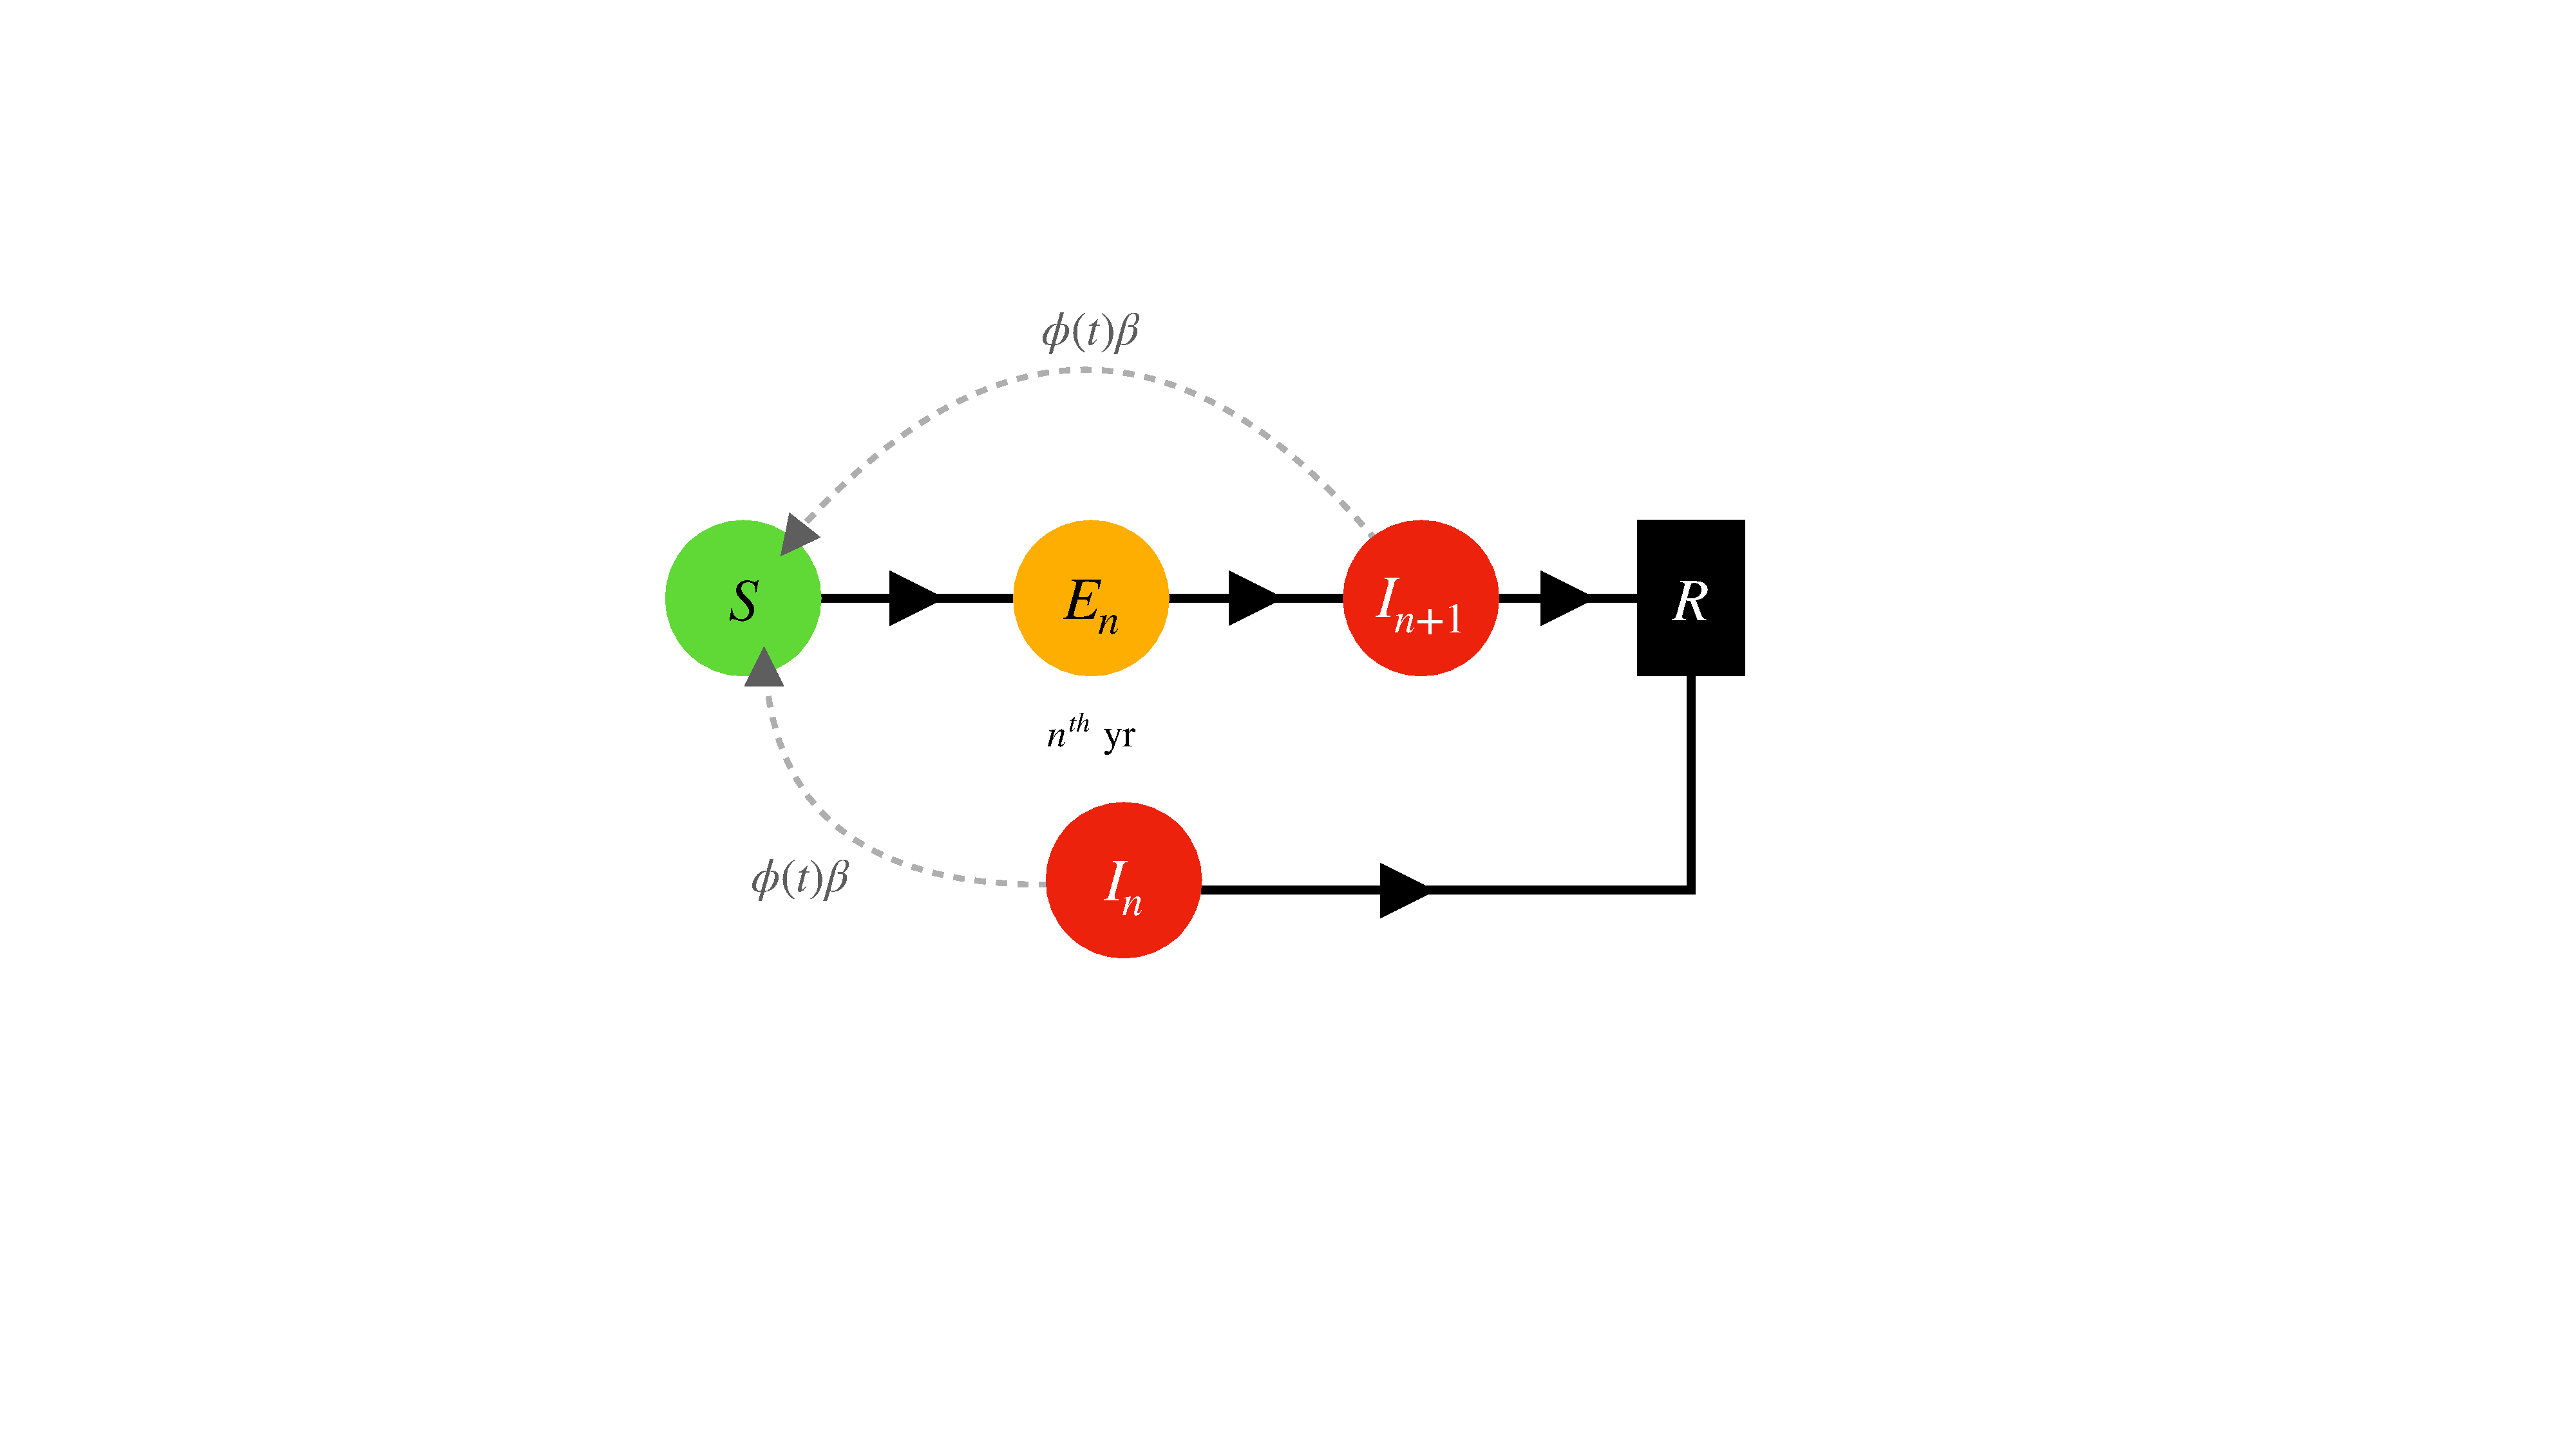
\includegraphics[scale=0.30]{chapter6/figures/fig1.pdf}
    \caption{The $SEIR$ model of ash dieback. In year $n$ of an outbreak, an infectious tree may cause a transition $S\rightarrow E_n$, depicted by the bottom dashed grey arrow. A tree that becomes latently infected in year $n$ will lead to an infectious tree in year $n+1$. Eventually, all infected ash are removed without the possibility of recovery.}
    \label{fig:SEIR-transitions}
\end{figure}

As define here, an ash tree transitions into the infectious compartment when leaf shedding begins in Autumn. A Gaussian distribution centred in November with a two-week standard deviation represents this in the model. This particular choice of standard deviation, although best-estimated, is ultimately ill-informed. However, because infected ash do not produce any secondary infections until the following summer, we can afford some degree of flexibility modelling the exact timing of transitions between $E_{n}\rightarrow I_{n+1}$; this flexibility is demonstrated in-depth later on.

Once in the infectious compartment, an infected ash tree will not give rise to any secondary infections until summer when fruiting bodies produce their spores on dead leaf litter. Thus, infectivity is now time-dependent and can be captured by a 'sporulation' function $\phi(t)$. Sporulation functions have been investigated in the context of a time-varying infectivity parameter \cite{time-varying-infectivity}. In the case of ADB, the function $\phi(t)$ is used to mirror the life cycle of ADB where new secondary infections only arise during the summertime sporulation \cite{https://doi.org/10.1111/mpp.12073}. That is, non-zero from June until September, and zero otherwise\footnote{Variations in ADB sporulation have been noted between European countries \cite{https://doi.org/10.1111/mpp.12073}, along with the potential for early-onset sporulation in the face of favourable environmental conditions. Although, the most generally agreed upon sporulation period is thought to be from June to September.}.

To model dispersal, a thin-tailed Gaussian was considered alongside a fat-tailed inverse power-law distribution\textemdash see table \ref{tab:SEIR-model}. A probability of transition $S_x \rightarrow E_x$ for Gaussian and inverse power-law respectively, can be seen to follow:
\begin{equation}
    Pr(S_{x} \rightarrow E_{x} ;\ I_{x^{\prime}} ) = \beta  \phi(T) \exp\Big[\frac{-r^2}{2\ell^2_{ga}}\Big] 
\end{equation}
\begin{equation}
    Pr(S_{x} \rightarrow E_{x} ;\ I_{x^{\prime}} ) = \beta \phi(T) (1 - r/\ell_{pl})^{-a}
\end{equation}
where $\phi(t)$ is a time-dependant function reflecting the seasonal life-cycle of ADB (Two sporulation functions are considered, the precise functional form is discussed in-depth below.) and $r$ is the distance between $S_x$ and $I_{x^\prime}$. Thus, the inclusion of an exposed category, together with a sporulation function, constrain the dynamics of ADB whereby: A) infected ash may display symptoms but crucially not disperse any infectious material B) ash may shed infected leaves in Autumn/winter, and thereby disperse infected material, but not lead to any secondary infections until the following summer.

Finally, the last transition to consider is from infected to removed $I_{n}\rightarrow R$. Given a $95\%$ mortality rate, ADB can be regarded as lethal. Therefore, once an ash tree becomes infected, an eventual transition to the $R$ compartment is assumed with a probability of one\footnote{Interestingly, edge-cases can contradict this assumption. For example, a sufficiently large quantity of inoculum deposited on ash leaves can result in leaf shed before the infection has the chance to spread throughout the tree \cite{https://doi.org/10.1111/mpp.12073}.}. As a first approximation, infected ash were chosen to have exponentially distributed life-times with a mean of five years, see table \ref{tab:SEIR-model}. 

The precise probability distribution describing $I_{n}\rightarrow R$ is, to my knowledge, non-existent in the literature. Although, observations of mortality ratios after years of infection provided some guidance towards an approximate time-scale. In particular, reports of $5\%$ mortality after two years of infection \cite{kessler2012dieback}, $75\%$ mortality within five years \cite{langer2015ash} and no observations of infected ash surviving beyond $15$ years \cite{wylder2018evidence}. However, as discussed in detail later, the main results of this chapter depend on time-scales below the mean infection life-time. So once again, there is some degree of flexibility in the precise time-scale of $I_{n}\rightarrow R$.


% subdividing compartments in this manner could also provide an easier implementation to hosts which become more infectious, through a greater production of spores, as the infectious cycle continues not to mention particular periods of environmental unsuitability.
% 
 
\subsection{Dispersal parameterisation}

Dispersal was informed by data collected in France by \cite{grosdidier2018tracking}. The field study conducted by \cite{grosdidier2018tracking} provide estimates for dispersal parameters by fitting data against a Gaussian and inverse power-law kernels. Notably, the authors studied dispersal at two different spatial scales, local and regional, \textcolor{red}{on the order of $1\mathrm{km}$, to $10-100 \mathrm{km}$ respectively}. For a review on the importance of scale, see chapter \ref{chapter2:litreview}. The experimental data analysed by \cite{grosdidier2018tracking} tracked ADB spores about known sources of infection. Although data on spore depositions does not necessarily correspond to a new infection, it sheds essential light on the spatial scale of ADB dispersal. 
\begin{figure}
    \centering
    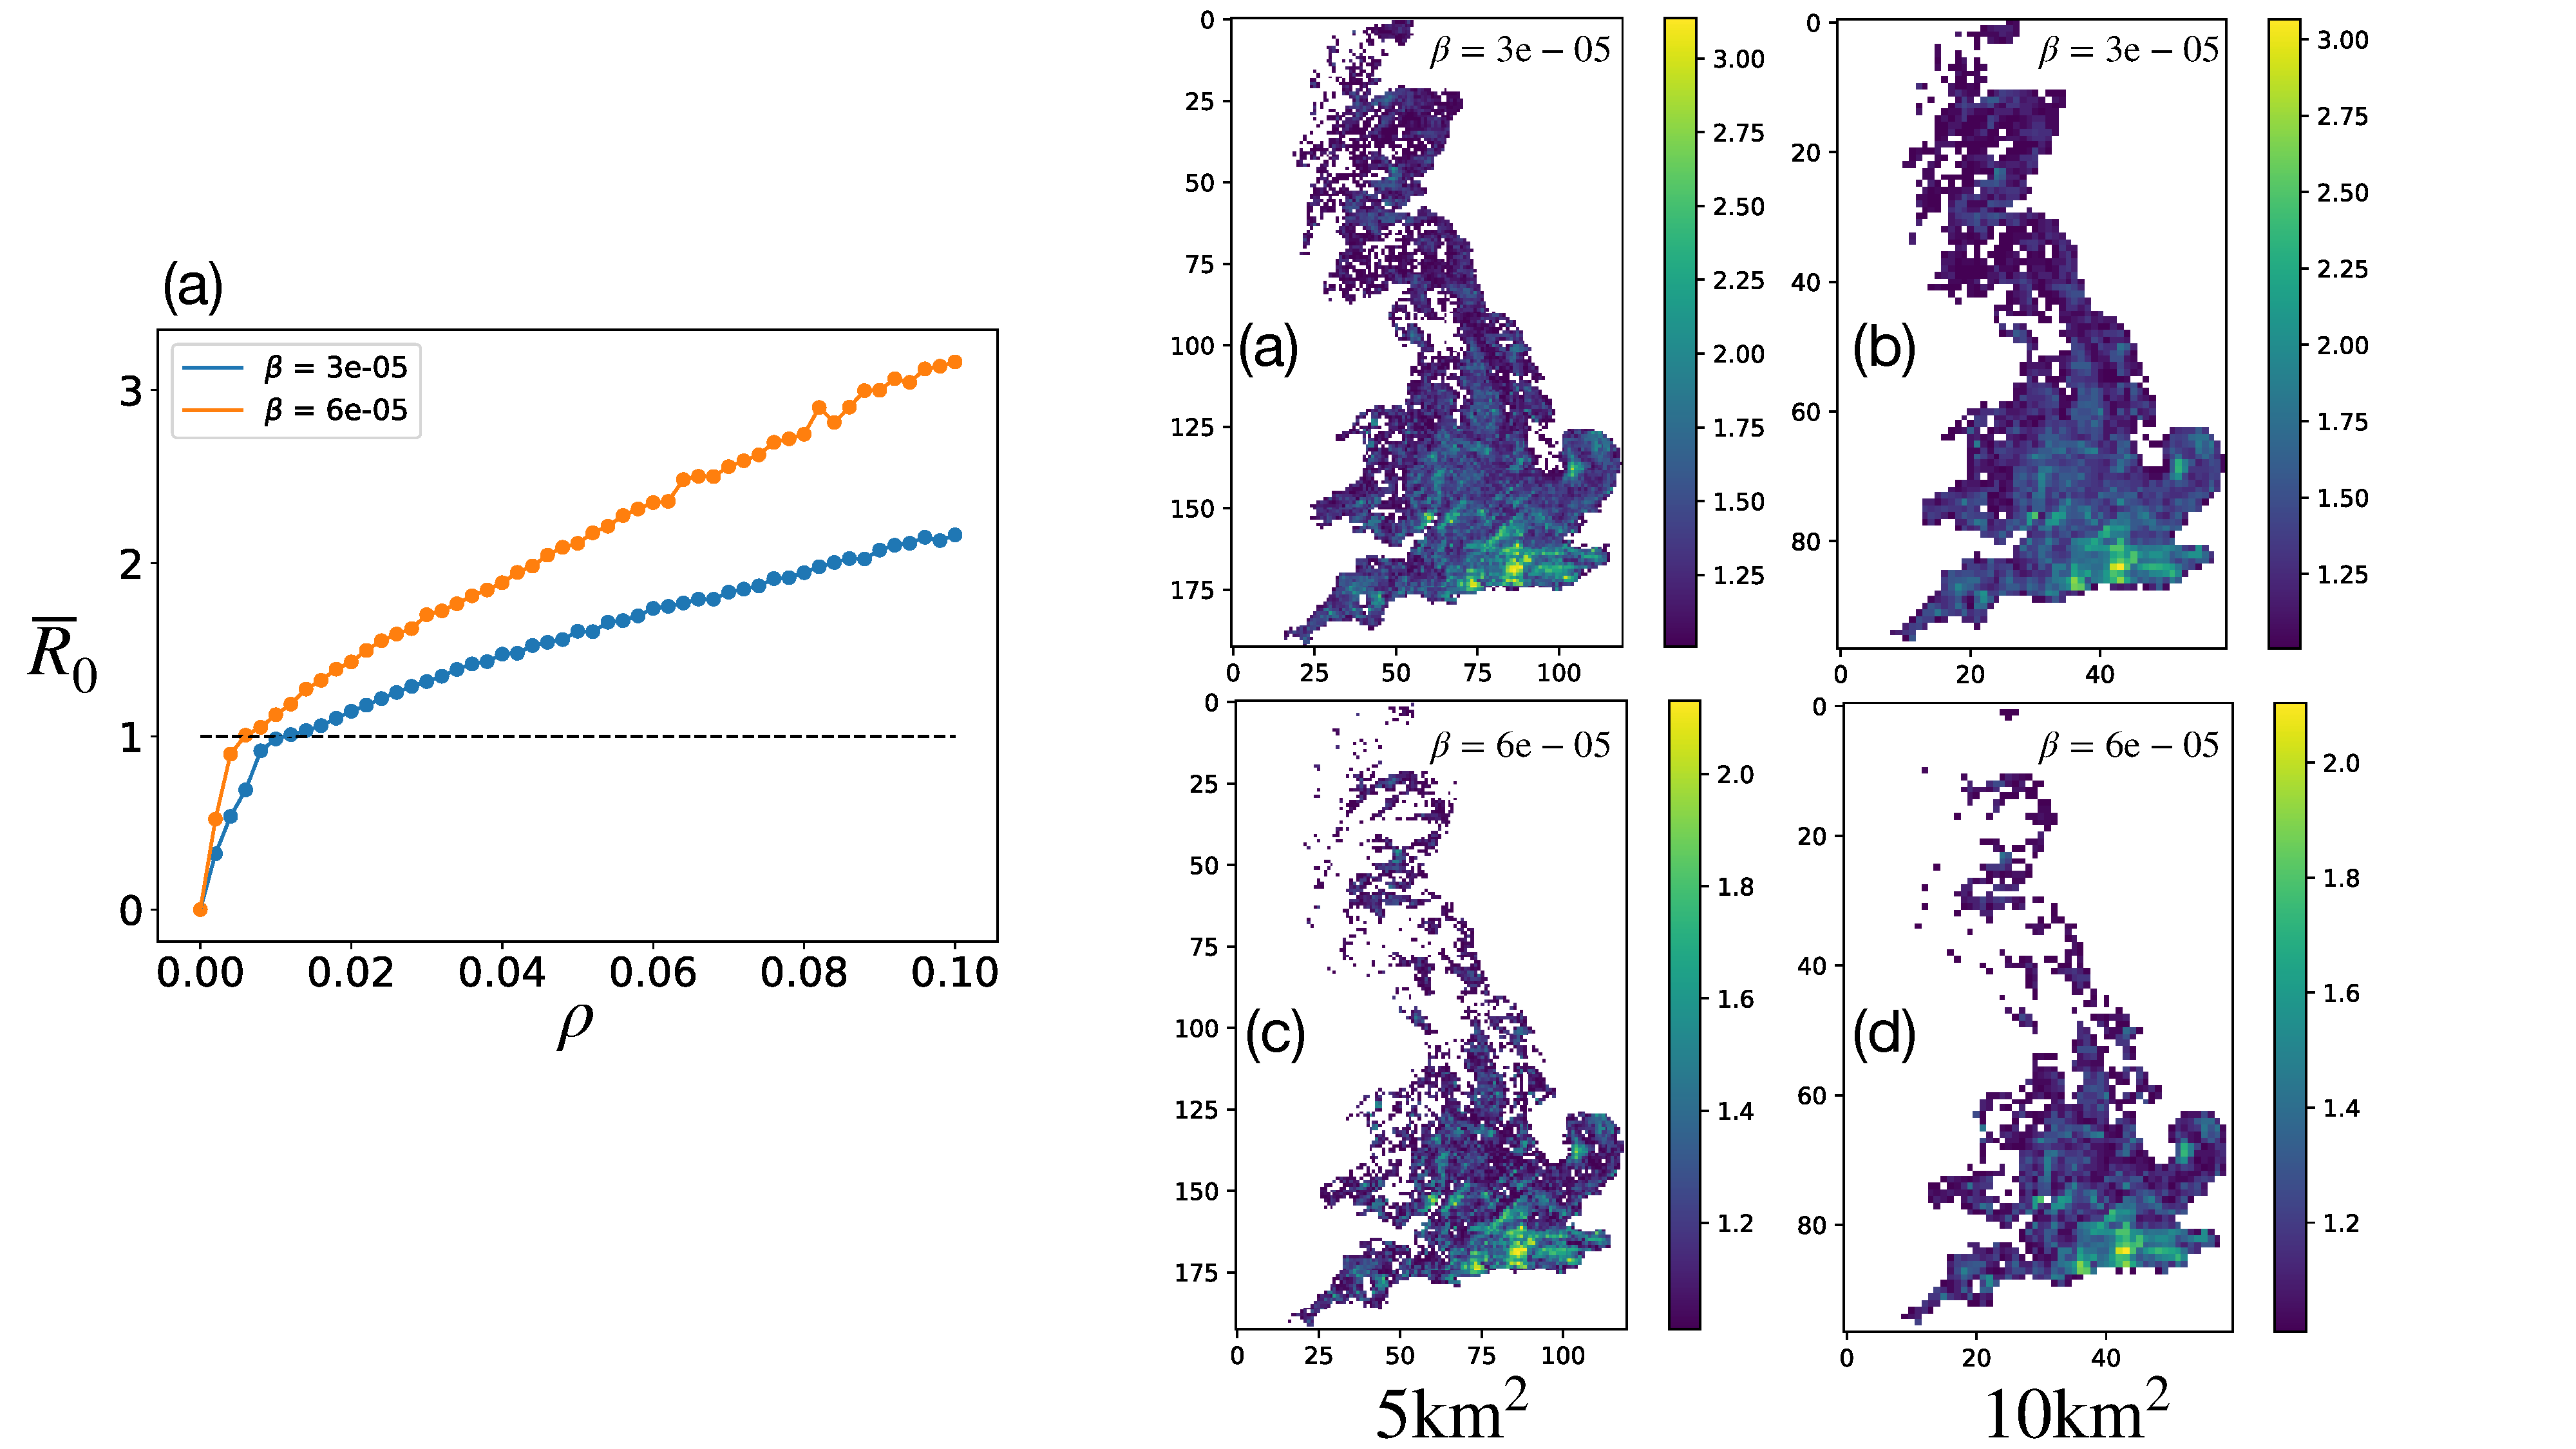
\includegraphics[scale=0.25]{chapter6/figures/fig2.pdf}
    \caption{Dispersal gradients at the local spatial scale, parameters are informed by the work of \cite{grosdidier2018tracking}. The authors provide estimates for Gaussian and inverse power-law kernels: $\ell_{ga} = 195\mathrm{m}$ and ($\ell_{pl} = 205\mathrm{m}$, $a=3.3$) respectively, where $a$ represents the inverse power-law exponent.}
    \label{fig:dispersal-parameterisation}
\end{figure}

Given that the spatial scale in the $SEIR$ model is small, at a  resolution of $5\mathrm{m} \times 5\mathrm{m}$, a decision was made to parameterise dispersal with the local-level dispersal values given by \cite{grosdidier2018tracking}. See table \ref{tab:SEIR-model} an Fig\ref{fig:dispersal-parameterisation}. This decision supposes that the spread of ADB in Great Britain is comparative to the spread of ADB in France. Nonetheless, there is a noticeable difference in the French climate, landscape and, importantly, wind patterns. % references
Notwithstanding these differences, it stands to reason that dispersal parameters, if measured over a smaller, local spatial scale, would be less pronounced. 

Lastly, the regional-scale dispersal analysed by \cite{grosdidier2018tracking}, measured over spatial scales of $10$-$100\ \mathrm{km}$, is thought to contain artefacts of LDD by human-mediated transport. The regional spread of ADB though LDD is, therefore, beyond the scope of the present chapter\textemdash a discussion of LDD will conclude this chapter and lead us to chapter into chapter \ref{ch7:pde}.


% Q: what is the relationship between the mortality ratio (or final fraction of infected hosts) ? 
% If R0 was considered over a larger time-scale, host-regrowth would need to be integrated into the model
% Furthermore, measuring R0 over a larger time-scale could over, or underestimate, the degree to which a response would need to be undertaken in the response time-window. 
% a basic reproduction number $R_0$ is defined for the first life-cycle of the pathogen.
% Moreover, data over a relatively short time scale is typically all that is available when making decisions about control, not to mention the added complexity of incorporating host-regrowth–which becomes an important factor over longer time scales–and so, the constraint of computing R0 over longer time scales is relaxed. 
%  We develop the simplest implementation possible, namely, where R_0 is measured over one pathogen life-cycle, and the course of infection for each host follows the same process with perfect fidelity. This lies in stark contrast to a realistic scenario whereby different hosts show considerable differences.

% \begin{itemize}
%     \item see for a review on how R0 is calculated \cite{perspectives-on-r0}, we use method x in order to estimate and inform R0
%     \item $R_0$ is a complex function which changes in time, to this end, the next generation operator is used to derive a value for $R_0$ \cite{doi:10.1098/rsif.2009.0386}. In order to inform the value of $R_0$ we do xy and
%     \item Although it is hard to enforce a true $R_0$ value, the most important feature introduced from the definition is a threshold from which we can see if a local invasion is likely to take place.
%     \item Since the number of susceptible hosts is fixed, without replacement, the number of susceptible hosts will continually decrease in time in the case of an epidemic. Given the strong spatial component in the model we expect that measuring $R_0$ as-per this definition will give an under-estimate for later times when few susceptible trees remain. Likewise, for earlier times when susceptible neighbours are plentiful $R_0$ will yield an upper estimate for the pathogen. In order to characterise the pathogen in this model, we take the upper bound defined between the $1^{st}-2^{nd}$ generations. This simplification represents a worst-case scenario and the mean value of $R_0$ would be lower for later times when there are less trees available to infect. But most importantly, the threshold of transmission $R_0>1$ is reliable captured \textit{during the initial stage of infection}.
%     \item $R_0$ can be fully characterised by a growth rate \cite{R0-construct}. That is, the growth factor per generation.
% \end{itemize}

\section{Seasonal $SEIR$ model behaviour}

In section \ref{sec:infection-dynamics}, the details of sporulation were omitted. For now, the simplest form of sporulation is adopted:
\begin{equation}
\phi(t) = 
\begin{array}{cc}
  \{ & 
    \begin{array}{cc}
      1 & t\in [\mathrm{June},\ \mathrm{September}] \\
      0 &  \mathrm{elsewhere}
    \end{array}
\end{array}
\end{equation}

\textcolor{red}{
The $SEIR$ model behaviour over $10$ years is shown in Figure \ref{fig:SEIR-spread} for Gaussian and power-law dispersal kernels. The simulations shown in Figure \ref{fig:SEIR-spread} were run using the average tree density for ash in Great Britain $\overline{\rho = 0.017}$ using canopy cover data from \cite{hill.data}. Furthermore, the domain size in Figure \ref{fig:SEIR-spread} was taken to be $2\mathrm{km}\times2\mathrm{km}$.}

\textbf{
\textcolor{red}{
The comparison between three different $\beta$ values paint an alarming picture, namely that a Gaussian spread gives rise to a more infectious pathogen, shown most clearly in Figures (a, b). This wrong for a number of reasons, goes against well established literature \cite{WEBIDEMICS} and would undoubtedly get pulled up by reviewers.}}

\textcolor{red}{
Gaussian dispersal has a higher $R_0$ in the immediate vicinity of infected trees, but crucially has a lower $R_0$ for further distances. One could then expect $R_0$ to saturate faster for Gaussian spreed, whereas for power law, an infectious tree has a larger neighborhood and will take longer to fill up with infectious trees. Therefore, I would power-law to have a higher $R_0$ than Gaussian based on spatial arguments. I have not seen this argument in the literature and could make for an interesting discussion point. Some interesting literature for $R_0$ in crop disease can be seen here \cite{mikaberidze2016invasiveness} and $R_0$ spatial maps here.}
\cite{R0-perc-ref}.

\textcolor{red}{This discrepancy between dispersal kernels is caused by the unnormalised Gaussian kernel in Figure \ref{fig:dispersal-parameterisation} having a larger area underneath the curve and thus integrating to a larger number. Of course, we could give Gaussian kernels a smaller $\beta$, which we are free to do because it is a probability and has no physical meaning. However, needing to change $\beta$ in order to compare Gaussian and power-law kernels is complicated, unintuitive and confusing.}

\begin{figure}
    \centering
    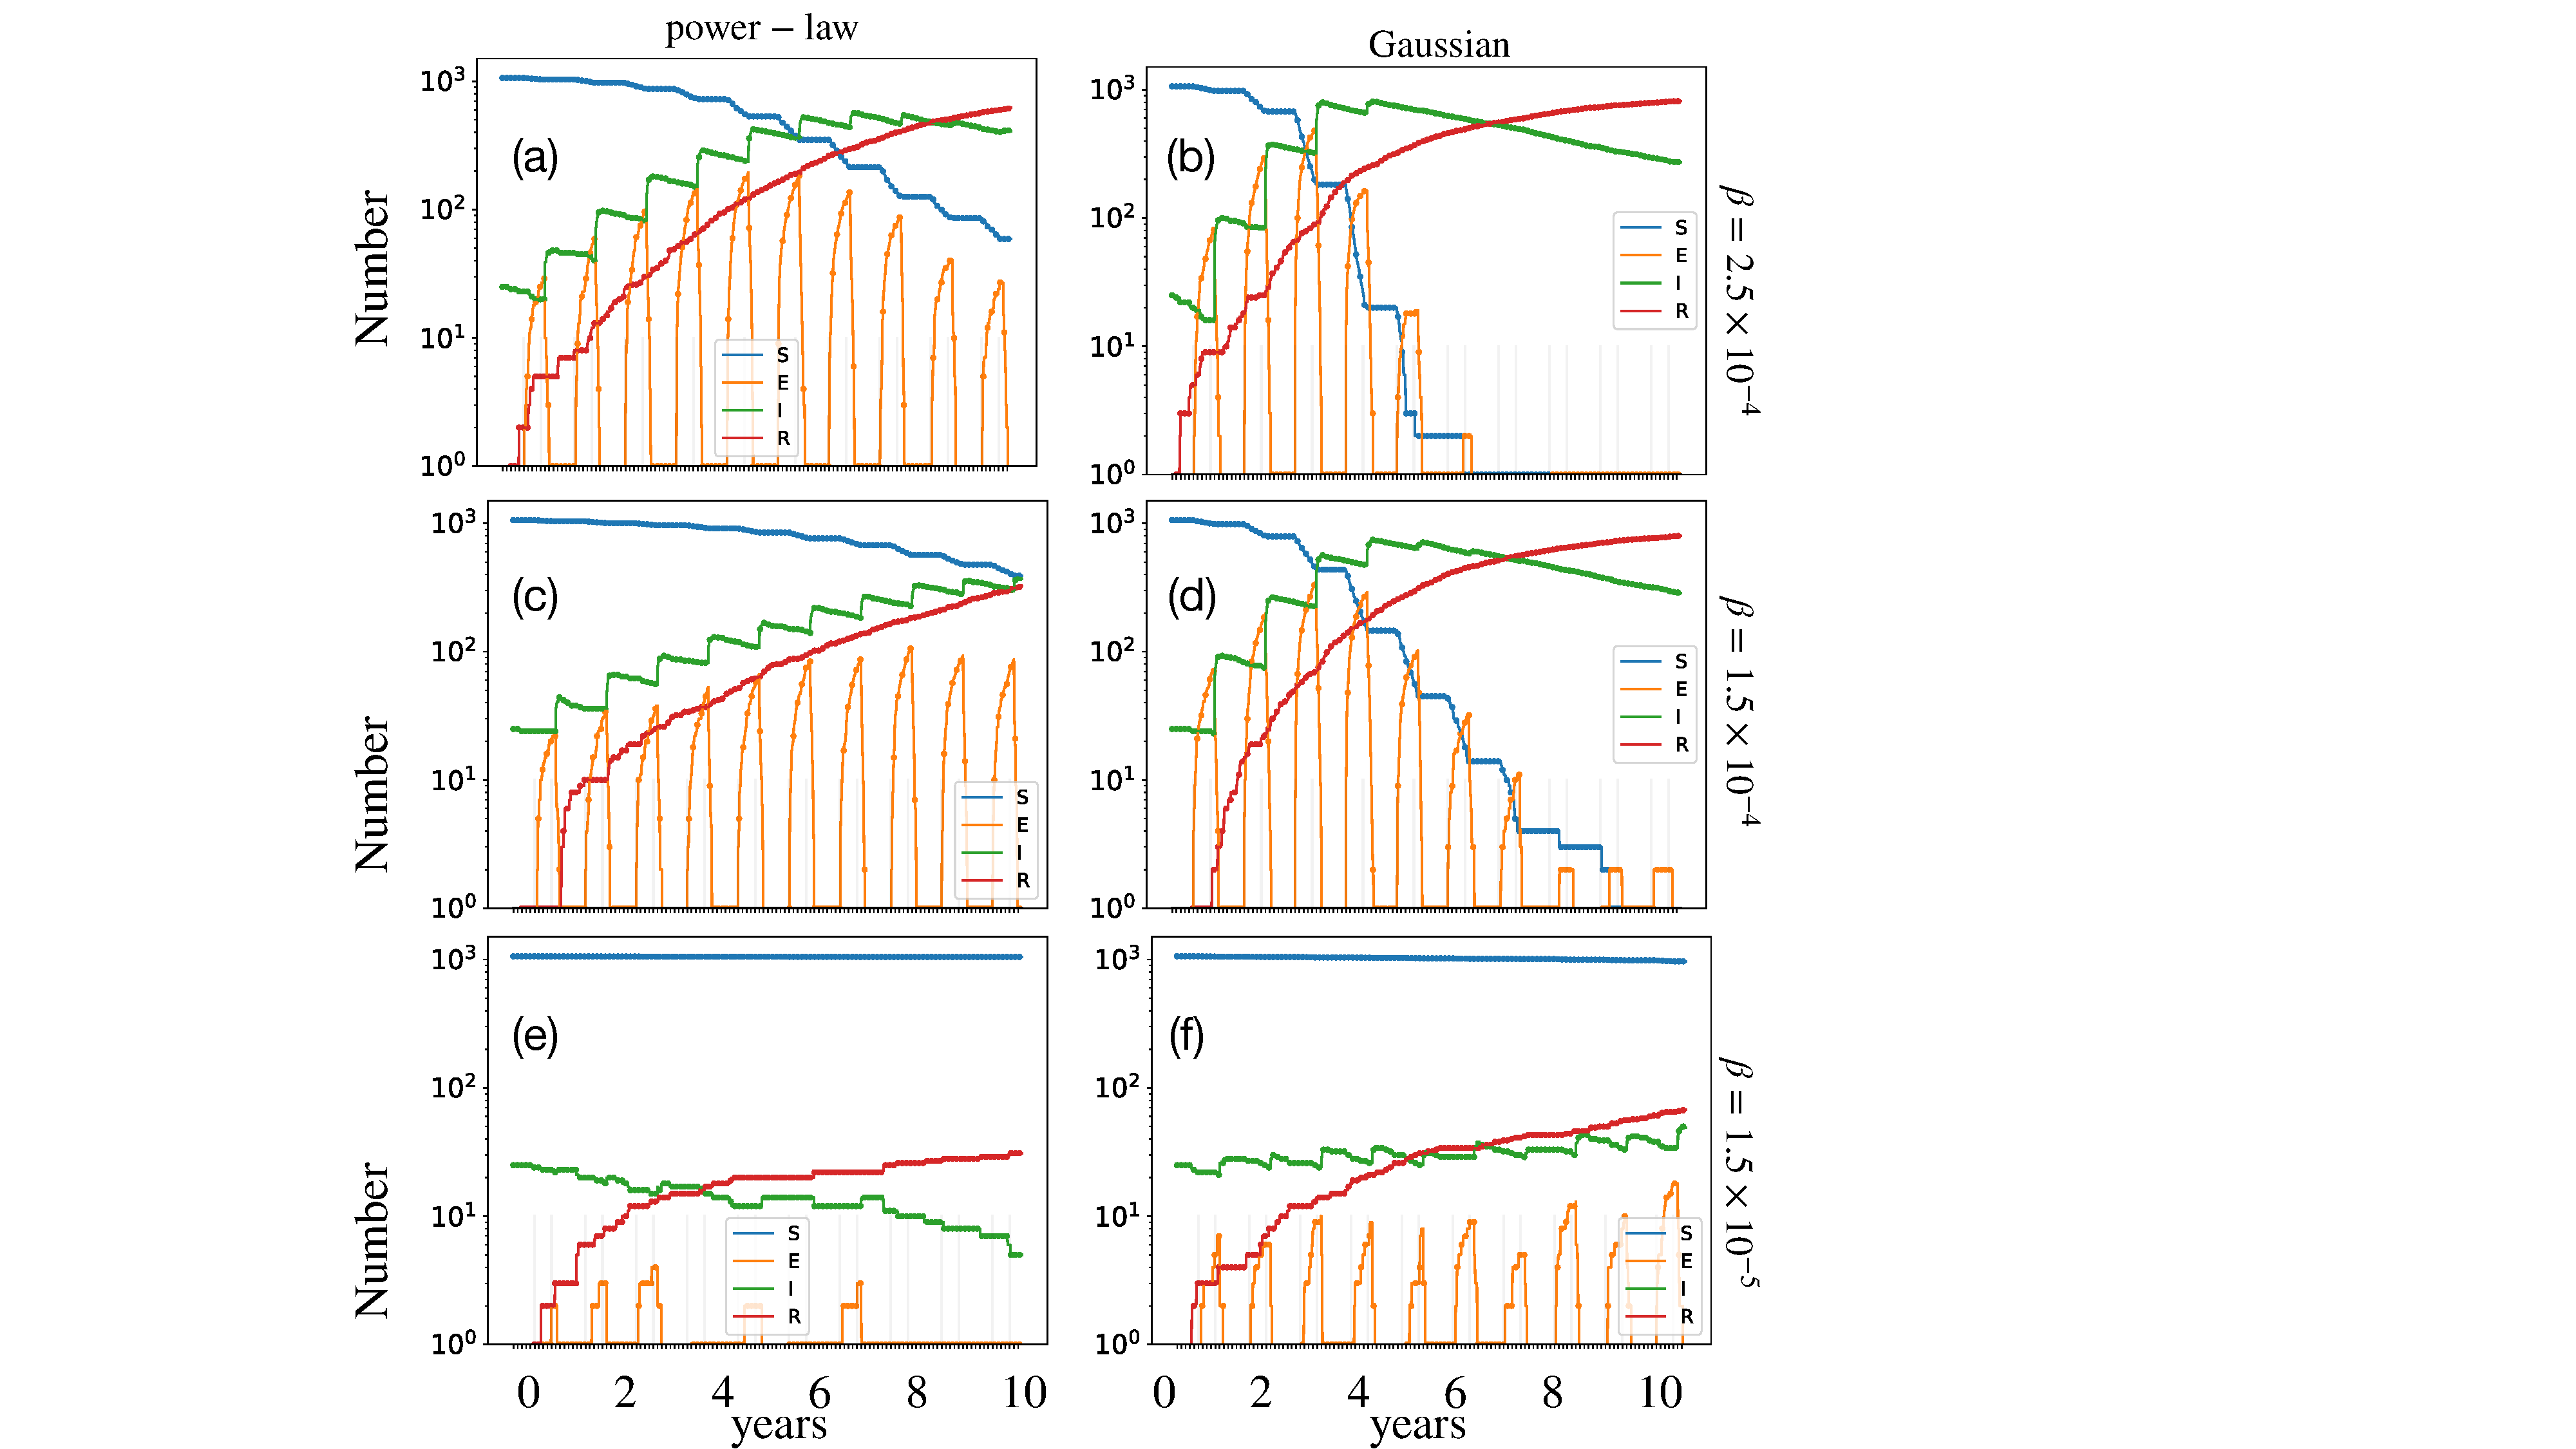
\includegraphics[scale=0.35]{chapter6/figures/fig4-seir-2.pdf}
    \caption{The $SEIR$ model behavior over ten years for the average ash density $\overline{\rho} = 0.017$ in a $2 \mathrm{km}\times 2\mathrm{km}$ domain.}
    \label{fig:SEIR-spread}
\end{figure}



\section{Defining an $R_0$}

Before the $SEIR$ model can be investigated, a measure of the pathogens ability to invade must be defined. For epidemic systems this usually comes in the form of a reproduction number $R_0$. There are, however, various challenges involved in measuring $R_0$ when there are dispersal-mediated secondary infections and spatial structure, as explored in chapter \ref{ch5:dispersal-model}. Namely, the spatial extent and the time-scale of measurement are essential factors that must be taken into account. In particular, chapter \ref{ch5:dispersal-model} demonstrated that $R_0$ is a spatio-temporal function of various epidemiological parameters and measuring $R_0$ over different spatio-temporal scales can lead to different, sometimes miss leading, results for $R_0$. 

Defining $R_0$ for ADB is additionally complicated by the seasonal component of its life cycle, not to mention the range of scales over which it spreads. Given that new secondary infections occur during summertime sporulation, a seasonal average $R_S$ can be defined for the model on a yearly basis. The definition of $R_S$ for ADB can then be stated as:
\begin{defn}
for years $(1,2.,,n)$ a series of ratios $(R_{1},R_2,...,R_{n})$ measure the mean number of secondary infections produced by an infectious ash over the sporulation season
\end{defn}
where 'mean' refers to the contact-traced number of infections produced by an individual as per Fig\ref{fig:contact-trace}.

In this model, the seasonal average $R_S$ is likely to underestimates the true value of $R_0$. This follows from the fact an infected ash tree has on average a life time of five years. It is widely accepted that policy makers should act quickly to a control an epidemic, and this observation once again highlights the challenge for policy makers because measuring $R_0$ over five years is likely to be too a time frame.


% - Show three different values of beta, above below and at threshold, for ga vs pl 


%\subsection{Defining an R0 value}
% Show that R0 A) over the season B) the problem policy makers experience by not having 5 years to wait before estimates of R0 C) How to form a crude estimate for R0 based on the first season 

% \subsection{Towards $\beta$ parameter-matching}
% - using mortality/infection \% data over match beta against percentage infected

% \subsection{Persistence}
%  - use a 10 year simulation below seasonal threshold, to show that the pathogen can survive for long periods within an area


\subsection{Sporulation}

% discuss multiple sporulation functions

% A simple time-dependant function $\phi(T)$ takes the value of $1$ between the summer months of June - September, and $0$ otherwise thus reflecting the sporulation peak of \textit{Hymenoscyphus fraxineus} (HF). During these summer months, wind-borne dispersal occurs when fruiting bodies produce large numbers of ascospores. 


\section{Informed ash density maps}

Ash densities are parameterised by modelled ash abundance data provided by \cite{hill.data}. The canopy cover datasets produced by \cite{hill.data} combine a number of different data sources that cover parts of Great Britain, regression methods are then used to extrapolate canopy cover over the whole of Great Britain\footnote{Previously in chapter chapter \ref{fig:ch4_uk_spread}, the oak canopy cover dataset given by \cite{hill.data} was used in conjunction with the SLM toy model; the insights from doing this then motivated the construction of a generic $SIR$-based dispersal model in chapter \ref{ch5:dispersal-model}.}. Conveniently for the present chapter, ash happened to be among the most accurate data sets given by \cite{hill.data}. For a more in-depth description of the methods used by \cite{hill.data} and a review of host data in general, see chapter \ref{chapter:lit-rev}.

 Two modifications had to be made to the modelled ash canopy cover data in order to complement the $SEIR$ model. Initially, the data set had a resolution of $\mathrm{1km}\times \mathrm{1km}$ and units of hectares of canopy cover per kilometre-squared of land $\mathrm{ha/km^2}$. Firstly, the raw abundance values were re-scaled into a dimensionless tree density $\rho$. The same process was outlined in chapter \ref{ch5:dispersal-model} i.e. by converting the units $\mathrm{ha/km^2}$ to kilometre-squared of ash cover per kilometre-squared of land. 
 
\begin{figure}
    \centering
    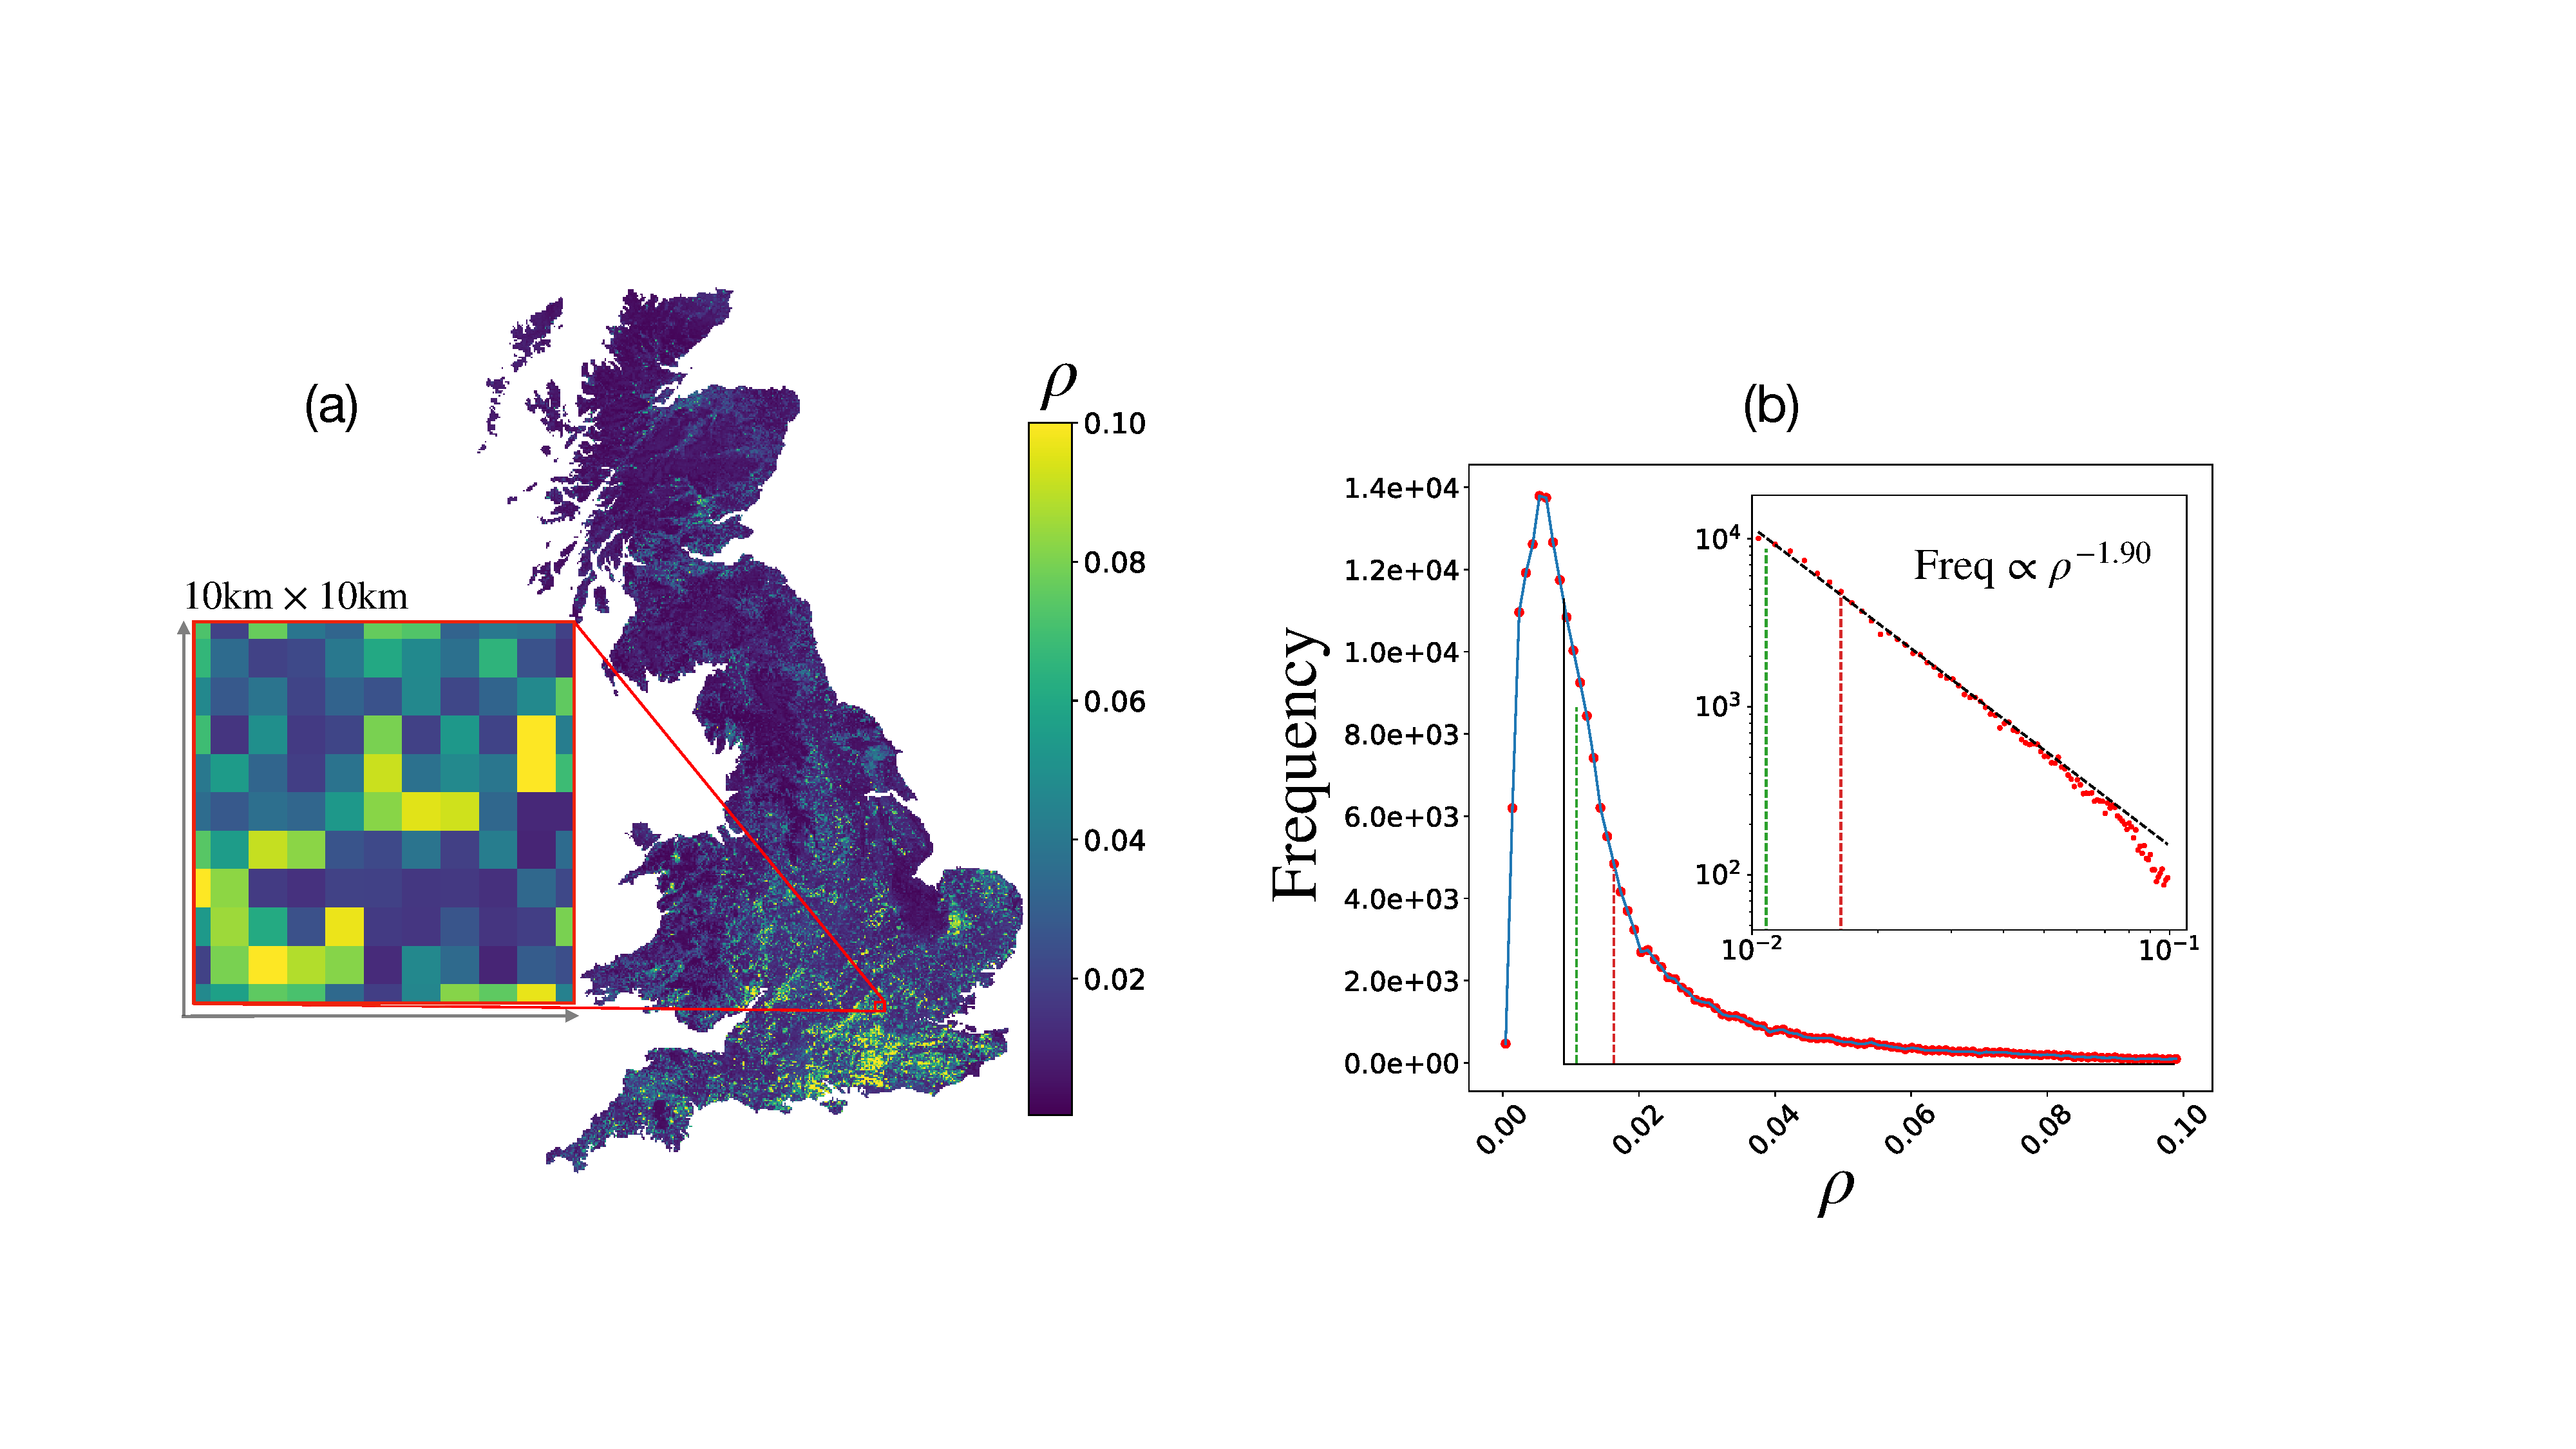
\includegraphics[scale=0.30]{chapter6/figures/fig3-ash-data.pdf}
    \caption{Ash canopy cover data, as modelled by \cite{hill.data}. (a) the original resolution of $1\mathrm{km} \times 1\mathrm{km}$ was re-scaled to $5\mathrm{km} \times 5\mathrm{km}$ (b) the distribution of ash density over the re-scaled map of Great Britain, the inset shows a power-law behaviour.} % Thi Figis a place holder. (a) and (b) need to reflect the $5\mathrm{km} \times 5\mathrm{km}$
    \label{fig:ash-host-data}
\end{figure}

Secondly, the resolution was re-scaled to $\mathrm{5km}\times \mathrm{5km}$, as shown in Fig\ref{fig:ash-host-data}(a). The purpose of re-scaling the map is a direct consequence of local wind-borne dispersal. In the local scale field study conducted by \cite{grosdidier2018tracking}, fungal spores were detected at a maximum distance of $500\mathrm{m}$ away from a known source of infection. If the domain consisted of $\mathrm{1km}\times \mathrm{1km}$ patches, it would be tangible for spores to disperse straight over individual patches and infect non-nearest neighbours. However, increasing the spatial extent of each pixel to $\mathrm{5km}\times \mathrm{5km}$ provides some level of assurance that at the local scale, wind-dispersed spores cannot jump over individual patches. There is always the possibility that spores travel larger distances, from mainland Europe to Great Britain, for example, \cite{freer2017tree, wylder2018evidence}. Nevertheless, this chapter is predicated on targeting dispersal at local scales, and such detail can be omitted for now.

The frequency distribution is shown in Fig\ref{fig:ash-host-data}(b) and reveals that the average density of ash in Great Britain is $\rho=0.017$. Furthermore, few locations support densities of $\rho=0.10$ and over\footnote{In the original $2.2\times 10^4$ $1\mathrm{km^2}$ data points, there were a handful of outlier points with densities in the interval $\rho \in [0.10, 0.30]$ which were excluded from the analysis.}.  Between the limits of $\rho \in [10^{-2}, 10^{-1}]$, the frequency distribution follows a power law of the form $\sim \rho ^{-k}$, as evident from the linearity on the logarithmic inset axes. The distribution had a fitted exponent of $k=1.90$, shown by the dashed black line. Intriguingly, this observation is suggestive of self-similarity in the data. Figure \ref{fig:ash-host-data}(a) shows that the south of England contains the highest concentration of high-density ash patches. Ash becomes progressively less abundant in Scotland and coastal locations in western Whales.

% \footnote{A review on the landscape epidemiology of ADB \cite{doi:10.1111/1365-2745.13383} concluded that the effect of host abundance in the neighborhood of ADB decayed with distance, according to an exponential distribution with scale parameter $200\mathrm{m}$. That is, the severity of ADB symptoms depended on the surrounding abundance of ash.} 
% 

\section{Constructing $R_0$-maps over Great Britain}
% discuss  projecting R0-maps
% Assumption, there is considerable genetic variation in susceptibility that varies between spatial location \cite{stocks2017first}

% In Figure\ref{fig:uk-mapping}, we can begin to identify heterogeneity and high-risk clusters of Ash. However, visualising which pixels connect to form large clusters is non-trivial. An image processing technique, `connected component analysis' (or CCA) \cite{CCA1, CCA2}, was used to identify and label susceptible clusters and simplify the $R_0$-map. This was performed using the function `label' from the Python-SciPy package `ndimage' \cite{scipy}. Doing so classified all susceptible (Moore) neighbours as connected members of the same cluster. \textcolor{red}{Figure \ref{fig:uk-mapping}(b) shows the top 10 largest $R_0$-clusters found in the map of Figure\ref{fig:uk-mapping}(a).}

% % Interpretation of clusters
% In this simplified interpretation, clusters represent a connected medium of Ash capable of supporting an epidemic, whereas regions below threshold act as barriers that inhibit the spread. Provided there is no long range dispersal (over $\mathrm{1km}$), a pathogen will not jump between clusters and will remain localised. Epidemic impact in this model will therefore correlate closely to cluster size as only large clusters have the potential of tending towards a nationwide spread of disease. Subsequent analysis will therefore concentrate on the largest susceptible clusters of Ash.\\

% \begin{figure}
%     \centering
%     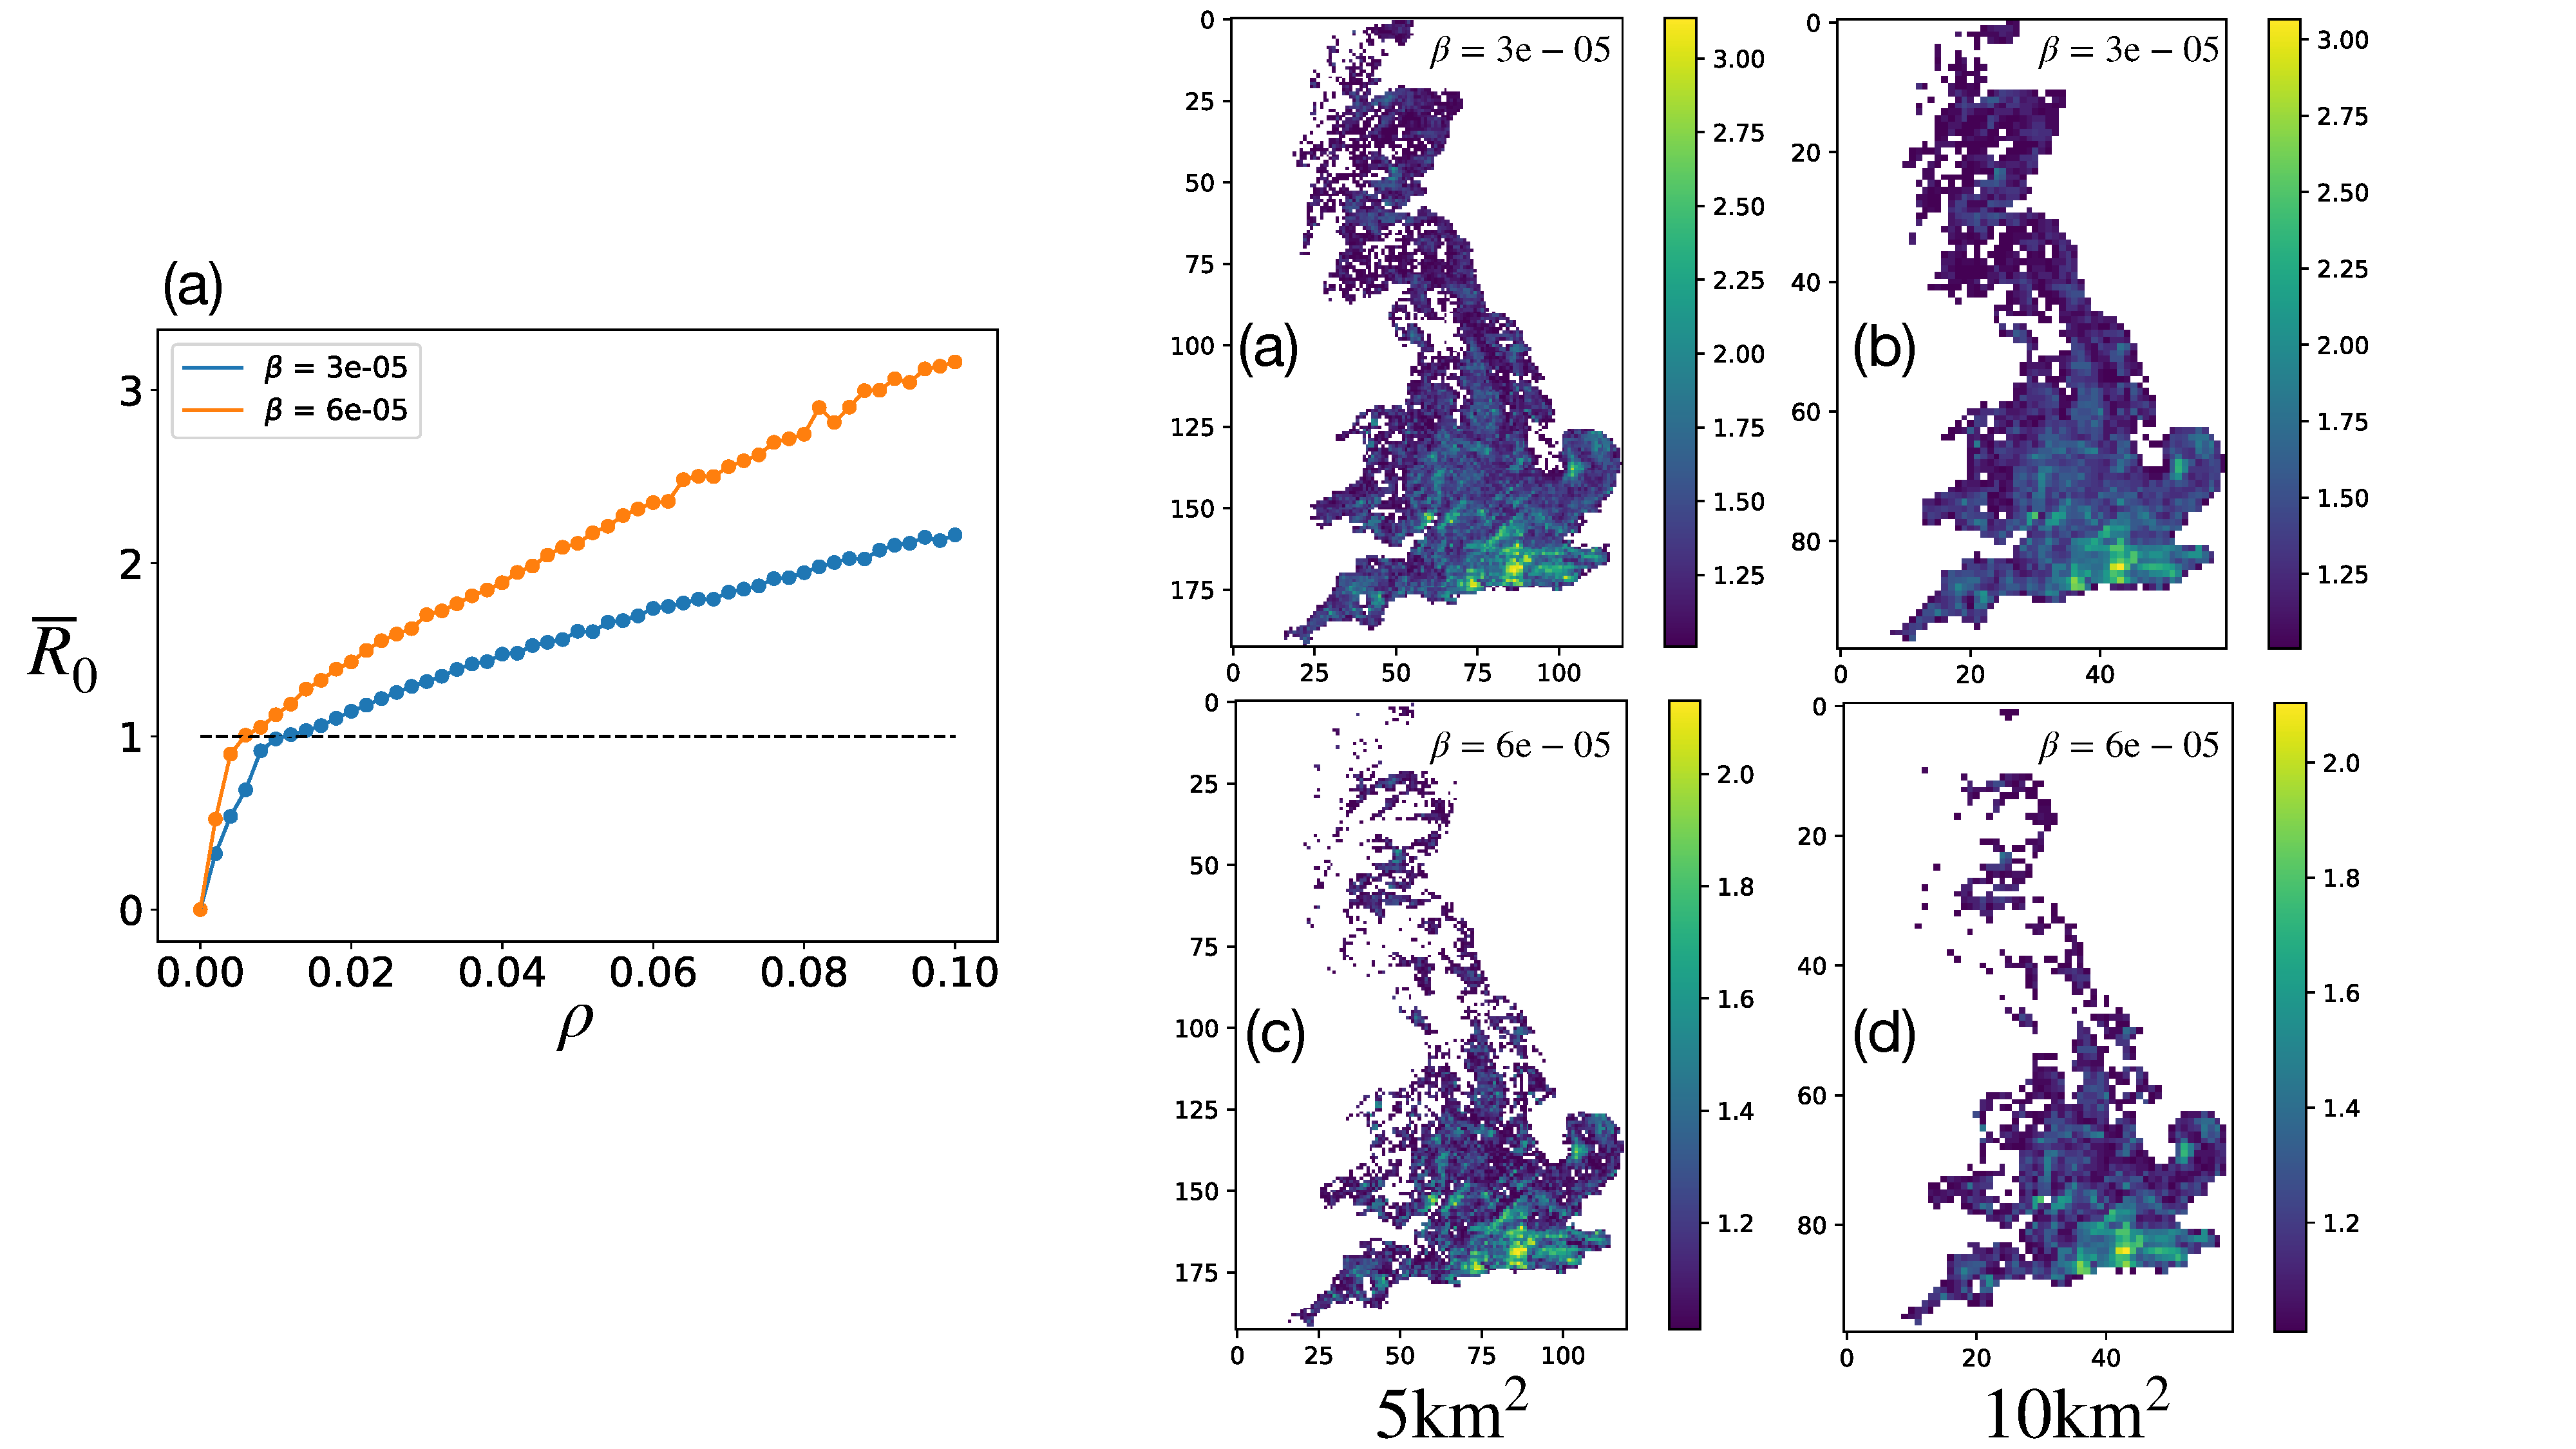
\includegraphics[scale=0.25]{chapter6/figures/fig4.pdf}
%       \caption{(a) Ensemble-averaged $R_0$ between two values of $\beta$, for Gaussian dispersal of $\ell=1.6\mathrm{km}$. (a-b) $R_0$-map for $\beta=3\mathrm{e}-05$, coarse-grained at $5$, $ 10\mathrm{km^2}$. (c-d) $R_0$-map for $\beta=6\mathrm{e}-05$.}
%     \label{fig:uk-mapping}
% \end{figure}

% % Linking R0 clusters to percolation theory
% The structure of connected $R_0$-clusters can be considered through the lens of a `\textit{percolation-like}' theory: if the $R_0$-map were homogeneous, a minimum number of susceptible (or `open' in percolation theory) positions defines a critical density. At the critical density, a `spanning' cluster is realised and percolates through the domain. In Figure\ref{fig:uk-mapping}(b), this picture is complicated by heterogeneity. Subsequently, we found connectedness inside a given cluster could depend on just a small number of `connecting points' which if removed, thinned below $\rho_c$, would lead to significant fragmentation and divide the cluster\footnote{An analogy to this idea can be found in the study of `conductive-insulator' percolation networks, with so called `\textit{hot-bonds}'. If broken, a \textit{single} hot bond can prevent the whole system from conducting \cite{RevModPhys.45.574, Herrmann_1984, hot-bond}. Although, in our analysis, a generalisation of this analogy is presented to include a set of \textit{multiple} hot-bonds.}.\\

% \textcolor{red}{Strictly speaking, the comparison with percolation theory breaks down on account of clustering in the $R_0$-map. That is, the susceptibility of a given pixel is likely dependent on its neighbours $R_0$-value. This contradicts classical percolation theory where lattice points are not correlated but exist independently of one another\textemdash much like the random-homogeneous distribution of trees presented in Section \ref{section:sgm-expo}. We precede by describing how these findings can be used to achieve efficient regional containment of an epidemic.\\}

\section{Optimal fragmentation of $R_0$-maps}

% Each cluster (denoted by $\mathbf{C}$) detected in the $R_0$-map represents a connected network of susceptible Ash where pathogen survival and spread is possible. The shape of each cluster is constrained by landscape topography and geography. If no control is attempted, all trees within a cluster are put at risk if one point in the cluster becomes infected. Given this, a control strategy is formulated by noting that removing specific positions of Ash (or breaking critical `links') via selective tree felling would efficiently break the cluster into two fragments. A technical explanation of the fragmentation algorithm is given in Appendix B.\\

% Cluster fragments define two disconnected `sub-clusters' (named $\mathbf{C_1}$ and $\mathbf{C_2}$). This eliminates risk for trees inside one sub-cluster and accomplishes control by regionally containing an epidemic inside a `confining cluster'. Ash trees inside the confining cluster are assumed to be removed by the pathogen while Ash trees inside the remaining sub-cluster survive and remain susceptible. If the number of felled trees is low in comparison to the number saved, then efficient control is achieved.\\

% The notion of fragmenting a cluster $\mathbf{C}$ into two sub-clusters $\mathbf{C_1}$ and $\mathbf{C_2}$ may be repeated $N$ times to produce a set of disconnected sub-clusters. After each fragmentation, sub-clusters were ranked according to the Ash population size they contained. This allowed the largest sub-cluster to be targeted in the next iteration. \textcolor{red}{Figure X} shows the largest cluster identified in the $R_0$-map (named $\mathbf{C_T}$) iteratively fragmented $N=5$ times culminating in six disconnected sub-clusters, depicted as the colour-filled regions from orange-green. The zoomed inset of $\mathbf{C_T}$ highlights the critically-connecting links found during each fragmentation.\\


% We assume the average Ash tree in the population covers an area of $\mathrm{25m^2}$ (giving a maximum of $400$ trees per hectare of canopy cover \cite{ash-tree2, ash-tree1}). Combining this assumption with the data permits us to estimate the number density of Ash trees per point and subsequently the population size of Ash contained inside each sub-cluster. Additionally, an estimate towards the number of felled trees can be formed, thus giving insight into the scale of resource expenditure. This is achieved by first finding the difference between $\rho_c$ and the density values of critical links (i.e. the level of required density reductions), then multiplying this by the number density.\\

% \textcolor{red}{Figure \ref{fig:result-cluster-reductions}(b)} shows the maximum sub-cluster population size in blue alongside the estimated number of trees needed to be felled in red. The largest sub-cluster continually decreased over $N=30$ iterations of fragmentation. Size reductions occurred more rapidly at first, starting from $\mathrm{3.5\times 10^7}$ trees and decreasing to $\mathrm{1.1\times 10^7}$ trees within $5$ iterations. By $N=30$, the rate of sub-cluster size reductions leveled off suggesting fragmentation in the field may tend towards diminishing returns on control efficiency. That is, larger values of $N$ produce smaller changes in the number of saved trees in proportion to the expenditure of resources needed to fell trees. This is demonstrated when the red and blue lines begin to approach each other, attaining comparable values.\\ 

% \textcolor{red}{Figure \ref{fig:result-cluster-reductions}(c)}, sub-cluster size reductions in $\mathbf{C_T}$ are shown alongside the $2^{nd}$ and $3^{rd}$ largest $R_0$-clusters on a log-log plot\textemdash from solid blue through to green. The straight lines indicate a power-law. The sub-cluster size reductions were fitted to a power-law of the form $f(x) = ax^{-k}$, shown by the corresponding dashed lines. Fitted parameter values of $a$ and $k$ represent the initial cluster population size and rate of decrease respectively. Importantly, all sub-cluster size reductions demonstrate an exponent of $k\sim 3/4$. In addition to the Ash species shown here, Conifer (\textit{Pseudotsuga menziesii}) and Beech (\textit{Fagus sylvatica}) were given by \cite{hill.data} and were used comparatively to test fragmentation. For each species considered, all iteratively fragmented clusters had similar exponent values, $k\sim 3/4$.\\


% \subsection{Towards epidemic control}
% % Main results figure 7
% Regional containment as a strategy of epidemic control was tested by considering outbreaks from different epicenters inside the target cluster $\mathbf{C_T}$. Starting from an epicenter, epidemic containment can be achieved in a variety of ways. \textcolor{red}{Figure \ref{fig:scenario-expo}} demonstrates this for a single epicenter marked by the black cross. The number of fragmentation iterations is varied from $N=1$ to $N=30$. For each step $N$, we identify which critical links, shown in red and denoted as $F$, should be felled below $\rho_c$ in order to define a confining sub-cluster around the epicenter. The population of saved Ash, illustrated in light grey, remains in state $S$ while all trees inside the confining sub-cluster, shown in dark grey, are assumed to transition into state $R$. By assessing the number of trees saved against the number of trees felled we can define a `payoff' ratio as $N_S/N_F$.\\

% A set of epicenters were defined in $\mathbf{C_T}$ (by identifying the center of mass for each sub-cluster when $\mathbf{C_T}$ was iteratively fragmented $N=30$ times). From $31$ different epicenters and $30$ iterations, $930$ containment scenarios were simulated. For some epicenters, typically in close proximity, containment looked identical up to $N$ iterations before a different payoff ratio was registered. Subsequently, less than $930$ unique data-points between $N_S$ and $N_F$ were found\textemdash shown in \textcolor{red}{Figure\ref{fig:result-culling-efficiency}}.\\

% The payoff ratios determined from the top $50$ performing containment scenarios were then ranked and plotted, shown in Figure\ref{fig:result-culling-efficiency}(a) by the blue line overlaid with a coloured scatter plot. For the purposes of our model, the payoff efficiency is shown alongside the corresponding number of felled trees in dashed grey. Payoff efficiencies begin to level off around $\mathrm{10^3}$ involving around $\mathrm{10^4}$ felled trees. In reality, this would be a challenge to accomplish in a reasonable time-frame. Figure\ref{fig:result-culling-efficiency}(b) shows a scatter plot of all the data, $N_S$ and $N_F$ are plotted with color corresponding to the payoff. The efficiency ranged over multiple orders of magnitude up to a maximum efficiency of $\mathrm{10^6}$. The top left quadrant of Figure \ref{fig:result-culling-efficiency}(b) represents viable scenarios where containment felling could be pragmatically implemented by policy makers with the greatest efficiency.\\

% A small number of exceedingly high payoff results were found. In Figure\ref{fig:result-culling-efficiency}(c), the top three ranking payoff scenarios are illustrated on the same map and reinforces the intuitive notion that epicenters around edge positions can be most efficiently contained. The zoomed inset highlights just $\mathrm{2\times 1km^2}$ Ash patches located at a single point of contact for the top ranked sub-cluster. Critical links for the best performing scenarios were all found in lower-density regions within the $R_0$-cluster and were easily fragmented with a low number of felled trees. This highlights the possibility that fragmentation is most easily achieved with tree felling through critically linking regions and demonstrates how regional variation in host density can be exploited for efficient control. 

\section{Chapter summary}

% Where we consider spatial structure and others have not
% - In this chapter, we focused on disrupting local-level dispersal by implementing control at landscape-level.
% -  In this chapter we undertook the ambitious task of scaling up a small-scale model, to large spatial distances covering GB, and developed a new approach to controlling the spread of disease.
% - introduce the regime of pathogen spread we are interested in, we are not modelling continental long-range spread via upper atmosphere, nor are we interested in long-range human trade networks. We are interested in dispersal at the local level whereby passive means of wind, soil and or insects/animals. 

These results are focused toward help policy makers implement informed decisions, about \textit{where} to control the spread of disease, based on spatial arguments, when budgets are low\textemdash as noted by \cite{time-varying-infectivity}. Our approach of spatially scaling small-scale epidemiological principles was conducted through computational, opposed to analytical, means. 

The article published by \cite{time-varying-infectivity} indicates the possibility of \textit{preferentially} controlling an area based on the final-sized epidemic. It goes without saying that areas of land that have the largest final sized epidemic are likely the most density populated. However, we outline the possibility it might be more beneficial to preferentially control an area based on its spatial location and how it couples to to neighbouring areas.

% The scaling up of our model
The scaling up of our model resembles a metapopulation model, now commonplace when modelling plant-based epidemics, but crucially our large-scale model is not dynamic. A dynamic large-scale model is indeed useful for the prediction of time-scales and the movement of disease-fronts movement; however, we suggest they might be at best less useful for optimised large-scale control, and at worse, nicely complemented by the approach we develop.

If early data through a particular region, with known data, was collected, it would be a relatively short step to fit the dispersal model and scale up the model over large distances given the seemingly simple relation to host density $\rho$.
% At the small scale we have a uniform population. However for larger scales we have considerable spatial heterogeneity.
% spatial-scale and control, over a multi-seasonal pathosystem, have been investigated for sugar beet in the UK, see \cite{doi:10.1146/annurev.phyto.45.062806.094357} for a review.

% On the SEIR model

The cyclic nature of the $SEIR$-type model constructed in this article can also find resemblance in the, well established body of literature, of crop-based epidemics. It is common-place for a field of crops to become infested, then at the end of the growing season be totally eradicated by virtue of harvesting % \cite{time-varying-infectivity} has 
% we contend the SnIEmR model, considered over one sporulation peak, is a simplistic implementation of the SEIR-based model needed to compute an invasion threshold that represent the infection dynamics ash dieback. 
% The SEIR-based model is made more flexible, and can be readily extended or adapted to incorporate more biological realism, by virtue of splitting the E and I into multiple compartments\textemdash this is frequently done in human and animal-based models \citations..

%- Although the main result of our work was conduced over one sporulation peak, or life-cycle of ash dieback, splitting the model into various compartments was a useful and necessary step towards developing accurate large-tree species. reference  \cite{https://doi.org/10.1111/ppa.12894} alludes to multiple exposed periods being useful

%- A quantity of interest that appears frequently in the literature is the initial growth rate $r$, that is the density-independent growth at the start of any epidemic.
% See \cite{ferrandino2012time} for a review on the time-scales and sporulation of plant-based diseases.

% Fitting data to the early phases of an epidemic has been shown to give large differences in the final-size epidemic, or severity \cite{time-varying-infectivity}. However, we are only interested in a pathogens ability to invade and this can be closely approximated by measuring R0 over the fist observation (\see appendix)

% The variability between the particular life-cycle history followed by hosts is thought to be an important factor to consider\cite{ferrandino2012time}, and we intentionally neglected this for the purpose of simplicity...

% Accurately modelling time-varying infectivity is difficult \cite{13-challenges}, and as such, we opted for parsimony.

% Main assumptions in the method: 
% 1) Assumptions about dispersal
Dispersal over small spatial-scale is thought to predominately occur passively through wind, however other means of dispersal exist such as soil and or insects. There are many pathways a pathogen can use to spread through a landscape, including long-range dispersal, mediated through either human-trade networks %
\cite{hulme2009trade, banks2015role, chapman2017global} or dispersal in the upper atmosphere \cite{westbrook1999atmospheric, isard2005principles}.  

% We assumed some regions can sustain an epidemic and some cannot, we assume that $R_0>1$ is the threshold separating these regimes.

% 2) Assumptions about R0
To our knowledge, $R_0$ has not been estimated for Ash dieback, or indeed for any large deciduous tree species, unlike for some crop-based pathogens \cite{segarra2001epidemic}. The lack of $R_0$-estimates made it hard to scrutinize which $\beta$-valued $R_0$-map would be likely to reflect reality. This gap in the body of literature is hardly surprising given the complexity of measuring time-varying infectivity rates \cite{13-challenges}. Thus, as it stands, our results hint-towards the utility of landscape-level control but come short of definitive proof.

% Looking at \cite{R0-perc-ref}, it makes me think our notion of $R_0$ is pretty simplistic. We only measure the local-level $R_0$. We do not consider $R_0$ from patch to patch. What scale we measure $R_0$ has a huge impact on what the result is. Could we rank land-patches not only on there local $R_0$ level, but also on the impact they have on there immediate neighbours ? This would, in theory be an improvement to the clustering algorithm.

% Improvements to the model:
% 1) The algorithm
% The algorithm to target not only the critically connecting patches, but also find fragmenting lines which minimise risk at the landscape-level ? Incorporating the local impact a particular patch may have on its neighbours.
% 2) Multi-year R0 analysis
% However, we .... xyz cover all basis of using a one-season approximation. <- this leads to a risk-based argument in which we could capture a 2nd-order R0 which does, xyz. We mainly interested in a pathogens ability to invade. 

% Analysis was aired towards simplicity, a more expansive study with e.g. more sophisticated sporulation functions could be the subject of future work.

% The most important message of our work was...
% The spatial and temporal scale of the control-strategy should match intrinsic spatial and temporal scale of the invasion. <- Hence R0 measured over one season. 


% our modelling approach and results are in their infancy,  

% Last remarks and future modelling work:
To our knowledge, there is a surprising lack of spatio-temporal ADB models exist in the literature, probably because of the significant challenges involved in containment. Although our findings are far from complete, it suggests the spread of ash dieback, between spatial locations, could be reduced by preferentially targeting sites to minimise epidemiological connectivity. Not surprisingly, more work will need to be done to ascertain the degree to which this strategy could impede the spread. 

% Crucially, future work will involve integrating LDD mechanisms into the model in order to understand the relative importance long vs local distance dispersal. We may speculate about the relative importance looking at figure x, whereby the maximum distance spread in season due to local-scale spread is xm/year, in stark contrast from the observed spread of 40-60km/yr.

% We cannot overstate the importance of LDD, and it is hard to say the degree to which targeting the local dispersal mechanism alone will inhibit the spread. We will revisit this question in future work, however, we contend that preferentially targeting diseased trees based on spatial location.....could help control epidemics with greater efficacy. 

% We may speculate how our result could aid the effort of choosing where to re-plant ash stands genetically engineered to be less susceptible; if re-planting efforts were undertaken in certain location.... <- speculative

% We may speculate about how persistent ash dieback would be, even if a large-scale control effort was undertaken

% There is evidence to suggest regional variation in mortality due to ash dieback \cite{stocks2017first}, this could be incorporated into the model...

% Our results support the call for more research to be undertaken into multi-scale dispersal, 

% Recently, it has been suggested that the dispersal-kernel of wind-borne pathogens might follow a scaling law \cite{https://doi.org/10.1111/jbi.13642}. The significance of such a finding would allow us to analyse the $R_0$-maps over much more flexible spatial scales. % Explain.

% This sentence is wrong, the cited paper makes an argument for the spatially-scaling up of dispersal kernels, which happens to still be useful paper to cite, re-phrase and re-frame accordingly.

% see \cite{ash-dieback-costs}, and the references therein (methodology excel spread sheet S1), for mortality references the latest findings suggest a mean mortality rate of 95%.



